% !TeX encoding = UTF-8
% !TeX program = xelatex
% !TeX spellcheck = en_US

\documentclass[degree=bachelor]{thuthesis}
  % 学位 degree:
  %   doctor | master | bachelor | postdoc
  % 学位类型 degree-type:
  %   academic(默认)| professional
  % 语言 language
  %   chinese(默认)| english
  % 字体库 fontset
  %   windows | mac | fandol | ubuntu
  % 建议终版使用 Windows 平台的字体编译


% 论文基本配置,加载宏包等全局配置
% !TeX root = ./thuthesis-example.tex

% 论文基本信息配置

\thusetup{
  %******************************
  % 注意:
  %   1. 配置里面不要出现空行
  %   2. 不需要的配置信息可以删除
  %   3. 建议先阅读文档中所有关于选项的说明
  %******************************
  %
  % 输出格式
  %   选择打印版(print)或用于提交的电子版(electronic),前者会插入空白页以便直接双面打印
  %
  output = print,
  %
  % 标题
  %   可使用“\\”命令手动控制换行
  %
  title  = {LXeTPC 和 HPGe 探测反应堆中微子-原子核相干弹性散射的实验灵敏度研究},
  title* = {An Introduction to \LaTeX{} Thesis Template of Tsinghua
            University v\version},
  %
  % 学位
  %   1. 学术型
  %      - 中文
  %        需注明所属的学科门类,例如:
  %        哲学、经济学、法学、教育学、文学、历史学、理学、工学、农学、医学、
  %        军事学、管理学、艺术学
  %      - 英文
  %        博士:Doctor of Philosophy
  %        硕士:
  %          哲学、文学、历史学、法学、教育学、艺术学门类,公共管理学科
  %          填写“Master of Arts“,其它填写“Master of Science”
  %   2. 专业型
  %      直接填写专业学位的名称,例如:
  %      教育博士、工程硕士等
  %      Doctor of Education, Master of Engineering
  %   3. 本科生不需要填写
  %
  degree-name  = {工学硕士},
  degree-name* = {Master of Science},
  %
  % 培养单位
  %   填写所属院系的全名
  %
  department = {工程物理系},
  %
  % 学科
  %   1. 学术型学位
  %      获得一级学科授权的学科填写一级学科名称,其他填写二级学科名称
  %   2. 工程硕士
  %      工程领域名称
  %   3. 其他专业型学位
  %      不填写此项
  %   4. 本科生填写专业名称,第二学位论文需标注“(第二学位)”
  %
  discipline  = {工程物理},
  discipline* = {Computer Science and Technology},
  %
  % 姓名
  %
  author  = {徐大成},
  author* = {Xue Ruini},
  %
  % 指导教师
  %   中文姓名和职称之间以英文逗号“,”分开,下同
  %
  supervisor  = {杨丽桃, 助理教授},
  supervisor* = {Professor Zheng Weimin},
  %
  % 副指导教师
  %
  associate-supervisor  = {高飞, 助理教授},
  associate-supervisor* = {Professor Chen Wenguang},
  %
  % 联合指导教师
  %
  % co-supervisor  = {某某某, 教授},
  % co-supervisor* = {Professor Mou Moumou},
  %
  % 日期
  %   使用 ISO 格式;默认为当前时间
  %
  % date = {2019-07-07},
  %
  % 是否在中文封面后的空白页生成书脊(默认 false)
  %
  include-spine = false,
  %
  % 密级和年限
  %   秘密, 机密, 绝密
  %
  % secret-level = {秘密},
  % secret-year  = {10},
  %
  % 博士后专有部分
  %
  % clc                = {分类号},
  % udc                = {UDC},
  % id                 = {编号},
  % discipline-level-1 = {计算机科学与技术},  % 流动站(一级学科)名称
  % discipline-level-2 = {系统结构},          % 专业(二级学科)名称
  % start-date         = {2011-07-01},        % 研究工作起始时间
}

% 载入所需的宏包

% 定理类环境宏包
\usepackage{amsthm}
% 也可以使用 ntheorem
% \usepackage[amsmath,thmmarks,hyperref]{ntheorem}

\thusetup{
  %
  % 数学字体
  % math-style = GB,  % GB | ISO | TeX
  math-font  = xits,  % sitx | xits | libertinus
}

% 可以使用 nomencl 生成符号和缩略语说明
% \usepackage{nomencl}
% \makenomenclature

% 表格加脚注
\usepackage{threeparttable}

% 表格中支持跨行
\usepackage{multirow}

% 固定宽度的表格。
% \usepackage{tabularx}

% 跨页表格
\usepackage{longtable}

% 算法
\usepackage{algorithm}
\usepackage{algorithmic}

% 量和单位
\usepackage{siunitx}

% 参考文献使用 BibTeX + natbib 宏包
% 顺序编码制
\usepackage[sort]{natbib}
\bibliographystyle{thuthesis-numeric}

% 著者-出版年制
% \usepackage{natbib}
% \bibliographystyle{thuthesis-author-year}

% 本科生参考文献的著录格式
% \usepackage[sort]{natbib}
% \bibliographystyle{thuthesis-bachelor}

% 参考文献使用 BibLaTeX 宏包
% \usepackage[style=thuthesis-numeric]{biblatex}
% \usepackage[style=thuthesis-author-year]{biblatex}
% \usepackage[style=apa]{biblatex}
% \usepackage[style=mla-new]{biblatex}
% 声明 BibLaTeX 的数据库
% \addbibresource{ref/refs.bib}

% 定义所有的图片文件在 figures 子目录下
\graphicspath{{figures/}}

% 数学命令
\makeatletter
\newcommand\dif{%  % 微分符号
  \mathop{}\!%
  \ifthu@math@style@TeX
    d%
  \else
    \mathrm{d}%
  \fi
}
\makeatother

% hyperref 宏包在最后调用
\usepackage{hyperref}

\thusetup{
  equation-number-separator = {-},
}
\usepackage{svg}


\begin{document}

% 封面
\maketitle

% 学位论文指导小组、公开评阅人和答辩委员会名单
% 本科生不需要
% \input{data/committee}

% 使用授权的说明
% \copyrightpage
% 将签字扫描后授权文件 scan-copyright.pdf 替换原始页面
\copyrightpage[file=scan-copyright.pdf]

\frontmatter
% !TeX root = ../thuthesis-example.tex

% 中英文摘要和关键字

\begin{abstract}
  中微子与原子核的相干弹性散射(CE$\nu$NS)是一种标准模型下的粒子物理过程。
  本文对以核反应堆作为中微子源、使用液氙时间投影室探测器和高纯锗探测器测量该过程的灵敏度进行了预测。
  通过设计建造一个极低阈值、极低本底并可在地面附近运行的液氙时间投影室。
  在信号所在能区,电子反冲本底预计可以压低至0.1$\left(\si{kg}\cdot\si{day}\cdot\si{keV}\right)^{-1}$水平,
  $\mu$子引起的核反冲本底可以压低至0.5$\left(\si{kg}\cdot\si{day}\right)^{-1}$水平。
  在一台堆芯热功率250$\si{GW}$商业发电反应堆附近运行一年,30千克量级的液氙时间投影室探测器预计探测到超过3000个CE$\nu$NS信号。
  通过设计建造一台本底水平与CDEX-10类似的5千克高纯锗探测器,在同等条件下,预计探测到超过1000个CE$\nu$NS信号。
  利用探测器到的CE$\nu$NS过程,两种探测器对中微子超标准模型有效相互作用和低动量转移下的弱混合角的测量将在类似实验中达到领先水平。

  % 关键词用“英文逗号”分隔,输出时会自动处理为正确的分隔符
  \thusetup{
    keywords = {中微子与原子核的相干弹性散射, 灵敏度预测, 本底模拟, 超标准模型有效相互作用},
  }
\end{abstract}

\begin{abstract*}
  An abstract of a dissertation is a summary and extraction of research work and contributions.
  Included in an abstract should be description of research topic and research objective, brief introduction to methodology and research process, and summary of conclusion and contributions of the research.
  An abstract should be characterized by independence and clarity and carry identical information with the dissertation.
  It should be such that the general idea and major contributions of the dissertation are conveyed without reading the dissertation.

  An abstract should be concise and to the point.
  It is a misunderstanding to make an abstract an outline of the dissertation and words “the first chapter”, “the second chapter” and the like should be avoided in the abstract.

  Keywords are terms used in a dissertation for indexing, reflecting core information of the dissertation.
  An abstract may contain a maximum of 5 keywords, with semi-colons used in between to separate one another.

  % Use comma as separator when inputting
  \thusetup{
    keywords* = {keyword 1, keyword 2, keyword 3, keyword 4, keyword 5},
  }
\end{abstract*}


% 目录
\tableofcontents

% 符号对照表
% !TeX root = ../thuthesis-example.tex

\begin{denotation}[3cm]
  \item[$E_\nu$] 反应堆中微子能量
  \item[$\epsilon$] 事件在探测器中沉积能量
  \item[$T_\mathrm{nr}$] 核反冲能量
  \item[$T_\mathrm{er}$] 电子反冲能量
  \item[$G_F$] 费米常数
  \item[$\theta_w$] Weinberg 角
  \item[$M$] 原子核质量
  \item[$N_\gamma$] 液氙中沉积能量产生光子个数
  \item[$N_e$] 液氙中沉积能量产生漂移电子个数
  \item[$L_y$] 液氙光产额
  \item[$Q_y$] 液氙电子产额
  \item[$N_\mathrm{hit}$] PMT阵列接收到的击中数目
  \item[$Q_F$] 淬灭因子
  \item[$E_\mu$] $\mu$子能量
\end{denotation}



% 也可以使用 nomencl 宏包,需要在导言区
% \usepackage{nomencl}
% \makenomenclature

% 在这里输出符号说明
% \printnomenclature[3cm]

% 在正文中的任意为都可以标题
% \nomenclature{PI}{聚酰亚胺}
% \nomenclature{MPI}{聚酰亚胺模型化合物,N-苯基邻苯酰亚胺}
% \nomenclature{PBI}{聚苯并咪唑}
% \nomenclature{MPBI}{聚苯并咪唑模型化合物,N-苯基苯并咪唑}
% \nomenclature{PY}{聚吡咙}
% \nomenclature{PMDA-BDA}{均苯四酸二酐与联苯四胺合成的聚吡咙薄膜}
% \nomenclature{MPY}{聚吡咙模型化合物}
% \nomenclature{As-PPT}{聚苯基不对称三嗪}
% \nomenclature{MAsPPT}{聚苯基不对称三嗪单模型化合物,3,5,6-三苯基-1,2,4-三嗪}
% \nomenclature{DMAsPPT}{聚苯基不对称三嗪双模型化合物(水解实验模型化合物)}
% \nomenclature{S-PPT}{聚苯基对称三嗪}
% \nomenclature{MSPPT}{聚苯基对称三嗪模型化合物,2,4,6-三苯基-1,3,5-三嗪}
% \nomenclature{PPQ}{聚苯基喹噁啉}
% \nomenclature{MPPQ}{聚苯基喹噁啉模型化合物,3,4-二苯基苯并二嗪}
% \nomenclature{HMPI}{聚酰亚胺模型化合物的质子化产物}
% \nomenclature{HMPY}{聚吡咙模型化合物的质子化产物}
% \nomenclature{HMPBI}{聚苯并咪唑模型化合物的质子化产物}
% \nomenclature{HMAsPPT}{聚苯基不对称三嗪模型化合物的质子化产物}
% \nomenclature{HMSPPT}{聚苯基对称三嗪模型化合物的质子化产物}
% \nomenclature{HMPPQ}{聚苯基喹噁啉模型化合物的质子化产物}
% \nomenclature{PDT}{热分解温度}
% \nomenclature{HPLC}{高效液相色谱(High Performance Liquid Chromatography)}
% \nomenclature{HPCE}{高效毛细管电泳色谱(High Performance Capillary lectrophoresis)}
% \nomenclature{LC-MS}{液相色谱-质谱联用(Liquid chromatography-Mass Spectrum)}
% \nomenclature{TIC}{总离子浓度(Total Ion Content)}
% \nomenclature{\textit{ab initio}}{基于第一原理的量子化学计算方法,常称从头算法}
% \nomenclature{DFT}{密度泛函理论(Density Functional Theory)}
% \nomenclature{$E_a$}{化学反应的活化能(Activation Energy)}
% \nomenclature{ZPE}{零点振动能(Zero Vibration Energy)}
% \nomenclature{PES}{势能面(Potential Energy Surface)}
% \nomenclature{TS}{过渡态(Transition State)}
% \nomenclature{TST}{过渡态理论(Transition State Theory)}
% \nomenclature{$\increment G^\neq$}{活化自由能(Activation Free Energy)}
% \nomenclature{$\kappa$}{传输系数(Transmission Coefficient)}
% \nomenclature{IRC}{内禀反应坐标(Intrinsic Reaction Coordinates)}
% \nomenclature{$\nu_i$}{虚频(Imaginary Frequency)}
% \nomenclature{ONIOM}{分层算法(Our own N-layered Integrated molecular Orbital and molecular Mechanics)}
% \nomenclature{SCF}{自洽场(Self-Consistent Field)}
% \nomenclature{SCRF}{自洽反应场(Self-Consistent Reaction Field)}



% 正文部分
\mainmatter
% !TeX root = ../main.tex

\chapter{引言}

\section{研究背景与方法}

中微子是一种标准模型中的轻子,主要参与弱相互作用,有三种``味''。
上世纪三十年代,为了解决$\beta$衰变中的能量守恒问题,中微子作为一种假想粒子被引入。
因为中微子与普通物质(原子核与电子)的作用截面极小以致于极难探测,
直到1956年,借助反应堆中微子的超高流强和精巧的探测器设计,
C.L.Cowan 与 F.Reines 才探测到反应堆放出的电子反中微子(electron antineutrino)与质子之间的逆$\beta$衰变(inverse beta decay, IBD)反应\cite{cowan_detection_1956}。
在标准模型中,中微子被预测为一种不带电的无质量费米子,但是在二十一世纪初,
超级神冈实验(Super-Kamiokande)\cite{collaboration_evidence_1998}与萨德伯里中微子观测实验(SNO)\cite{sno_collaboration_direct_2002}
对大气中微子和太阳中微子的观测结果表明,中微子会在三种``味''之间发生转换,这同时意味着中微子之间的质量差异。
这是中微子展现出超出标准模型预言性质的一个证据。

中微子与原子核的相干弹性散射(Coherent Elastic Neutrino-Nucleus Scattering, CE$\nu$NS)是一种中微子与原子核的相互作用。
当中微子通过中性流(neutral-current)与原子核散射时,会与原子核之间以 Z 玻色子(Z boson)交换动能和动量。
当交换的动量足够低时,Z 玻色子将视原子核为一个整体进行相互作用,结果是原子核获得了一个很小的动能。
但中微子与原子核整体反应导致反应截面急剧升高,使得CE$\nu$NS成为$\si{MeV}$中微子与物质的主要相互作用,也为我们提供了测量该极低能过程的机会。
作为一种典型的弱相互作用,CE$\nu$NS测量可以限制某些弱相互作用相关的参数,同时为超标准模型物理提供契机。
同时CE$\nu$NS是下一代暗物质直接测量实验的重要本底\cite{ohare_fog_2021},对CE$\nu$NS的研究也会辅助提升未来的暗物质实验精度。

2017年,COHERENT 合作组在美国橡树岭国家实验室的散裂中子源(The Spallation Neutron Source (SNS) at Oak Ridge National Laboratory)
上通过碘化铯($\mathrm{CsI}$)探测器首次以高置信度探测到了CE$\nu$NS过程。
我们计划设计建造一台30千克量级的液氙时间投影室(liquid xenon time projection chamber, LXeTPC)
或一台5千克的高纯锗(high purity Germanium, HPGe)探测器对反应堆电子反中微子进行探测。
相比于散裂中子源上中微子,反应堆中微子能量更低(不超过 10$\si{MeV}$),对其的测量是现有实验的良好补充。

在探测器的研制设计中,对探测器关键本底的研究和预测本底对实验灵敏度的影响至关重要。
不同于XENON、LZ等地下实验,地面运行的LXeTPC不具有山体屏蔽,宇宙线$\mu$子流强将上升几个数量级。
对$\mu$子穿过探测器的过程中产生额外本底的控制,是实验成功的关键因素之一。同时探测器材料中产生的本底也不可忽略。
我将建立一套本底模拟框架和一套灵敏度预测框架,重点研究$\mu$致本底和材料本底对实验的影响,并最终给出实验的灵敏度预测。

\section{论文结构与章节安排}

本文各章节组织如下:

第一章为引言。简单介绍研究背景和方法。

第二章为CE$\nu$NS的研究背景。主要介绍CE$\nu$NS的发生过程和现有实验对其的探测方法和进展。

第三章介绍探测器工作原理。从探测器工作原理和探测器特性的角度,介绍LXeTPC与HPGe探测器对物理信号的探测过程,这一部分为接下来的LXeTPC和HPGe上的信号模型研究提供支撑。

第四章创建信号模型。基于探测器的工作原理和以往对反应堆中微子的研究,创建两种探测器上的CE$\nu$NS信号模型。信号模型将作为灵敏度预测的关键输入。

第五章对关键本底进行模拟。建立LXeTPC实验本底的模拟框架,研究$\mu$致本底和材料本底的水平压低方法,研究结果将作为本底模型输入灵敏度预测框架。

第六章进行灵敏度预测。基于第四、五章的分析,建立灵敏度预测框架,以中微子超标准模型有效相互作用、低动量转移下的弱混合角和低能核反冲的光电产额为例预测探测器在模拟得到的本底水平下,对关键物理目标的探测能力。

第七章为总结和展望。本章总结测量CE$\nu$NS的灵敏度预测工作思路,并提出当前工作的局限性,为未来的相关工作提出展望。

% !TeX root = ../main.tex

\chapter{CE$\nu$NS探测研究背景}

\section{CE$\nu$NS过程}

\begin{figure}
    \centering
    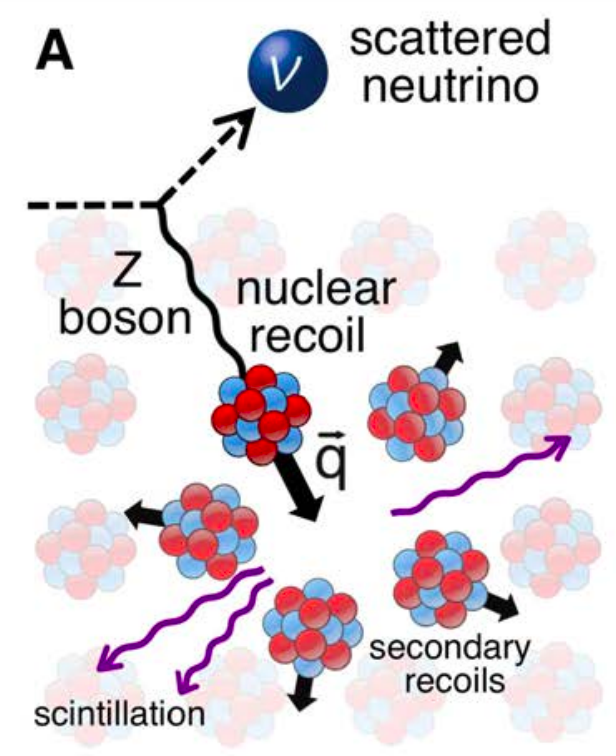
\includegraphics[width=0.4\linewidth]{figures/CEvNS_demo.png}
    \caption{\label{fig:cevns_demo} 中微子-原子核相干弹性散射示意图}
\end{figure}

CE$\nu$NS是中微子和原子核之间的弹性中性流相互作用,于1974年被首次预言提出\cite{freedman_coherent_1974,kopeliovich_isotopic_1974}。
如图\ref{fig:cevns_demo},中微子与原子核交换Z玻色子,同时也交换能量动量,产生核反冲(nuclear recoil, NR)。
被加速的原子核以散射光(scintillation)和后续碰撞(secondary recoils)的形式继续将能量沉积到周围的物质中,
最终这些信号被探测器记录到\cite{akimov_observation_2017}。在中微子和原子核交换Z玻色子的过程中,若动量转移足够小,
则原子核近似作为一个整体与中微子作用,作用截面近似与原子核中的中子个数的平方成正比关系。

\begin{align}
    \label{eq:cevns}
    \frac{\mathrm{d}\sigma(E_\nu)}{\mathrm{d}T} &= \frac{G_F^2 M}{2\pi}\left[(G_V+G_A)^2+(G_V-G_A)^2(1-\frac{T}{E_{\nu}})^2-(G_V^2-G_A^2)\frac{MT}{E_{\nu}^2}\right] \\
    G_V &= (g_V^p Z+g_V^n N)F^V(Q^2) \\
    G_A &= (g_A^p(Z_{+}-Z_{-})+g_A^n(N_{+}-N_{-}))F^A(Q^2) \\
    \label{eq:cevns_theta}
    g_V^p &= \rho_{\nu N}^{NC}(\frac{1}{2} - 2\hat{\kappa}_{\nu N}\sin^2\theta_W) + 2\lambda^{uL} + 2\lambda^{uR} + \lambda^{dL} + \lambda^{dR} \\
    g_V^n &= -\frac{1}{2}\rho_{\nu N}^{NC} + \lambda^{uL} + \lambda^{uR} + 2\lambda^{dL} + 2\lambda^{dR}
\end{align}

公式\ref*{eq:cevns}为具有特定能量$E_{\nu}$的电子反中微子与特定质量$M$的原子核的CE$\nu$NS微分截面,
其中$T$为末态原子核动能,$G_F$为费米常数(Fermi constant),本文中取为1.1664$\times10^{-5}\si{GeV}^{-2}$,$Q$为动量转移,$Z$和$N$分别为原子核内质子和中子的个数。
$F^V$和$F^A$为形状因子,在低动量转移下可以认为$F^V(Q^2)=F^A(Q^2)=1$\cite{lewin_review_1996},
$\rho_{\nu N}^{NC},\hat{\kappa}_{\nu N}$为弱电理论参数,
$\lambda^{uL},\lambda^{uR},\lambda^{dL},\lambda^{dR}$是辐射校正参数\cite{barranco_probing_2005}。
$Z_{\pm}$和$N_{\pm}$是原子核内自旋(spin)取向为上($+$)和下($-$)的质子和中子个数。

经过计算,$|g_V^p|\ll|g_V^n|$,所以在 $G_V$ 参数中起主要作用的因素是中子个数 $N$;
另一方面,根据原子核物理理论,对于偶偶核(even-even nucleus),即原子核内质子数$Z$和中子数$N$均为偶数时,$Z_{+}=Z_{-},N_{+}=N_{-}$。
届时 $G_A=0$,我们可以利用这一点将CE$\nu$NS截面简化。

\begin{align}
    \label{eq:cevns_even_even}
    \frac{\mathrm{d}\sigma(E_\nu)}{\mathrm{d}T} &= \frac{G_F^2 M}{2\pi}G_V^2\left[1+(1-\frac{T}{E_{\nu}})^2-\frac{MT}{E_{\nu}^2}\right] \\
    G_V &= (g_V^p Z+g_V^n N)F^V(Q^2)
\end{align}

公式\ref{eq:cevns_even_even}为CE$\nu$NS截面的的偶偶核简化形式。考虑到 $|g_V^p|\ll|g_V^n|$,则$G_V^2\approx N^2$,
最后可以近似得到$\frac{\mathrm{d}\sigma(E_\nu)}{\mathrm{d}T}\approx N^2$,对于非偶偶核,该式也近似成立。这正是CE$\nu$NS相干性的体现。

对于不同种类的核素,因为原子核的质量$M$不同,所以微分截面$\frac{\mathrm{d}\sigma(E_\nu)}{\mathrm{d}T}$不同。
将微分截面对原子核末态动能$T$积分,可以得到CE$\nu$NS总截面随着中微子能量$E_{\nu}$的变化关系。

\begin{figure}
    \centering
    \includesvg[width=0.6\linewidth]{figures/cross_section.svg}
    \caption{\label{fig:xsec_elements} CE$\nu$NS对各种核素的截面随着中微子能量$E_{\nu}$的变化关系}
\end{figure}

图\ref{fig:xsec_elements}中列举了几种探测器常用核素(元素)的CE$\nu$NS截面与$E_{\nu}$的关系。作为对比,图中还包括了IBD\cite{akimov_observation_2017}的截面以及中微子-电子相干弹性散射(neutrino-electron elastic scattering, E$\nu$ES)的截面随着$E_{\nu}$的变化。
几种截面都随着中微子能量升高而升高,但几种CE$\nu$NS截面始终高于IBD和与电子相互作用的截面。同时对于更重的元素,如$\mathrm{Xe}$,CE$\nu$NS截面相比于其他较轻元素更大。
从截面大小的角度看,CE$\nu$NS相比IBD更容易被探测;但是因为CE$\nu$NS的动量转移太小,且不同于IBD可以借助$\gamma$和中子进行事件标记,对CE$\nu$NS的成功探测远晚于IBD。
同时图\ref{fig:xsec_elements}也给提示我们选择探测器材料的思路:重元素的反应截面更大,对探测更有利。但是考虑到原子核末态动能也会随着元素质量数增加而偏向更低能量,
以及不同探测器介质下探测器技术和性能的差异,应综合考虑选择探测手段。

\section{CE$\nu$NS探测方法与进展}

2017年,COHERENT合作组在美国橡树岭实验室的散射中子源上使用$\mathrm{CsI}$以高置信度探测到了$\pi$介子(pion)衰变过程放出的中微子的CE$\nu$NS信号\cite{akimov_observation_2017}。
此后他们又并行开展了以其他手段进行CE$\nu$NS搜寻的实验,其中包括了HPGe、单相液氩(single phase LAr)探测器和碘化钠($\mathrm{NaI}$)。
虽然这些探测器的能量阈值不尽相同,但得益于散裂中子源中微子的较高能量($\mathcal{O}\left(10\si{MeV}\right)$),
CE$\nu$NS在这些探测器中的NR可以达到$\mathcal{O}\left(10\si{keV}\right)$,探测器阈值并不是实验成败的最关键因素。

目前有多个合作组及实验正在进行CE$\nu$NS探测研究,除COHERENT外均使用反应堆中微子作为中微子源。
表\ref{tab:experiments}列出了部分CE$\nu$NS探测研究的相关实验,但目前没有实验成功给出测量到反应堆中微子CE$\nu$NS的结果。

\begin{table}
  \centering
  \caption{从事CE$\nu$NS探测研究的相关实验}
  \begin{tabular}{ccc}
    \toprule
    实验名称 & 探测器材料 & 研究进展 \\
    \midrule
    COHERENT & $\mathrm{CsI,HPGe,LAr,NaI}$ & 进行中\cite{coherent_collaboration_monitoring_2022} \\
    CONUS & $\mathrm{Ge}$ 低温量能器 & 进行中\cite{conus_collaboration_novel_2021} \\
    CONNIE & $\mathrm{CCD}$ & 进行中\cite{connie_collaboration_search_2022} \\
    MINER & $\mathrm{Ge}$ 低温量能器 & 筹划中\cite{agnolet_background_2017} \\
    \bottomrule
  \end{tabular}
  \label{tab:experiments}
\end{table}

反应堆中微子CE$\nu$NS的低动量转移特性要求探测器实现极低阈值和低能区域的极低本底。
类似的要求也在在相关领域,如暗物质直接探测,成为探测器关键技术。低质量暗物质,如$\mathcal{O}\left(1\si{GeV}\right)$大质量弱相互作用粒子(Weakly interacting massive particles, WIMP)对探测器原子核的核反冲动量转移也在几个$\si{keV}$量级。
目前流行的暗物质探测技术中,LXeTPC和HPGe探测器均取得了较先进的成果。用于探测WIMP的探测器技术同样可以应用到同为核反冲信号的CE$\nu$NS探测中。
因反应堆均在地面附近,若设计建造一台能够在地面正常运行的LXeTPC或HPGe探测器,则有可能实现对反应堆中微子CE$\nu$NS的探测。

% !TeX root = ../main.tex

\chapter{LXeTPC与HPGe探测器的工作原理}

\section{LXeTPC的工作原理}

\section{地面运行的LXeTPC探测器设计}

\section{HPGe探测器的工作原理}

% !TeX root = ../main.tex

\chapter{CE$\nu$NS探测信号模型}

本章将分析反应堆中微子的来源和能谱,以探测器响应为基础建立实验中的信号模型。

\section{反应堆中微子的CE$\nu$NS}

典型的热中子堆(thermal-neutron reactor)中99.7\%以上的反应堆中微子来自于四种主要裂变核素子核(裂变碎片)的衰变:
${}^{235}\mathrm{U},{}^{238}\mathrm{U},{}^{239}\mathrm{Pu},{}^{241}\mathrm{Pu}$\cite{juno_collaboration_tao_2020}。
反应堆中可裂变核素均为富中子核素,其裂变碎片也是富中子核素,可以发生$\beta$衰变放出电子($\beta$射线)和电子反中微子。
每一次核裂变后会伴随约6次$\beta$衰变和中微子发射,热中子堆每吉瓦($10^{9}\si{W},\si{GW}$)热功率将每秒产生$2\times10^{20}$个电子反中微子。
这些中微子的能谱是几千种裂变碎片的$\beta$衰变中微子能谱的叠加,见图\ref{fig:fission}。裂变产物的复杂性对于精确地计算反应堆中微子能谱是不利的。

\begin{figure}
  \begin{subfigure}{.3\textwidth}
    \centering
    \includesvg[width=1.0\linewidth]{figures/Nuclear_fission.svg}
    \caption{\label{fig:nuclear_fission} 典型的${}^{235}\mathrm{U}$裂变过程}
  \end{subfigure}
  \begin{subfigure}{.7\textwidth}
    \centering
    \includesvg[width=1.0\linewidth]{figures/fission_yield.svg}
    \caption{\label{fig:fission_yield} ${}^{235}\mathrm{U}$和${}^{239}\mathrm{Pu}$的热中子裂变产额}
  \end{subfigure}
  \caption{\label{fig:fission} 热中子堆中的裂变过程。典型裂变核素${}^{235}\mathrm{U}$的产物,如${}^{92}\mathrm{Kr}$和${}^{141}\mathrm{Ba}$均为$\beta$衰变核素,见图\subref{fig:nuclear_fission};裂变碎片成分十分复杂,热中子裂变条件下,${}^{235}\mathrm{U}$和${}^{239}\mathrm{Pu}$裂变碎片的质量与产额关系中,碎片质量将以裂变核素质量的一半为轴,几乎左右对称,并形成两个峰\cite{crouch_fission-product_1977},见图\subref{fig:fission_yield}。}
\end{figure}

目前有两种反应堆中微子能谱模型。2011年前,最常用的反应堆中微子能谱为ILL-Vogel模型,其中${}^{235}\mathrm{U}$、${}^{239}\mathrm{Pu}$和${}^{241}\mathrm{Pu}$的
能谱反推自1980年代在ILL(the Institut Laue-Langevin)的裂变产物$\beta$能谱测量\cite{von_feilitzsch_experimental_1982,schreckenbach_determination_1985,hahn_antineutrino_1989},
因${}^{238}\mathrm{U}$裂变主要由快中子引发,难以直接测量,其中微子能谱来自P.Vogel的理论计算\cite{p_vogel_neutrino_1989}。
ILL-Vogel模型与2011年前的反应堆中微子实验的结果吻合\cite{an_improved_2017}。
2011年后P.Huber和T.A.Mueller等人引入了更精细的理论计算\cite{huber_determination_2011,mueller_improved_2011},称为Huber-Mueller模型,
得到的中微子能谱相对于测量结果有超出。

在灵敏度预测中高能(超过2$\si{MeV}$)中微子的能谱$s_i(E_\nu)$输入($i=1\cdots4$,遍历四种裂变核素),将使用Huber-Mueller模型,其中${}^{235}\mathrm{U}$、${}^{239}\mathrm{Pu}$和${}^{241}\mathrm{Pu}$参考P.Huber的计算结果\cite{huber_determination_2011},${}^{238}\mathrm{U}$参考T.A.Mueller的计算结果\cite{mueller_improved_2011};
在低能($0-2\si{MeV}$)区域,将使用P.Vogel的理论计算能谱\cite{p_vogel_neutrino_1989},见图\ref{fig:neutrino_energy_spectrum}。本文中将反应堆将只以裂变产物$\beta$衰变放出的电子反中微子作为中微子源。

\begin{figure}
    \centering
    \includesvg[width=0.7\linewidth]{figures/neutrino_energy_spectrum.svg}
    \caption{\label{fig:neutrino_energy_spectrum} 灵敏度预测中使用的各种核素的中微子能谱,
    因逆$\beta$衰变反应有约$1.8\si{MeV}$的阈值,所以虽然低能中微子占总流强的主要部分,但未被Daya Bay等反应堆中微子实验测量到\cite{an_improved_2017}。}
\end{figure}

为了计算反应堆中微子的总能谱和总流强,需要引入裂变核素每次裂变的平均释放能量$e_i$,已有较精确的理论计算\cite{ma_improved_2013},见表\ref{tab:per_fission}:

\begin{table}
  \centering
  \caption{四种主要裂变核素每次裂变释放的平均能量和裂变份额}
  \begin{tabular}{c|c|c}
    \toprule
    核素 & $e_i(\si{MeV})$ & $f_i$ \\
    \midrule
    ${}^{235}\mathrm{U}$ & 202.36 & 0.561 \\
    ${}^{238}\mathrm{U}$ & 205.99 & 0.076 \\
    ${}^{239}\mathrm{Pu}$ & 211.12 & 0.307 \\
    ${}^{241}\mathrm{Pu}$ & 214.26 & 0.056 \\
    \bottomrule
  \end{tabular}
  \label{tab:per_fission}
\end{table}

有了以上基础,反应堆中微子的能谱定义为:

\begin{align}
    \label{eq:sum_spectrum}
    \phi\left(E_\nu,t\right) &= \frac{W(t)}{\sum_i f_i(t)e_i}\sum_i f_i(t)s_i(E_\nu)
\end{align}

其中$t$为反应堆运行时间,$W(t)$为反应堆运行功率,其与堆芯实际运行状态有关\cite{juno_collaboration_tao_2020};
$f_i(t)$为裂变份额(fission fraction),指四种核素的裂变次数在总裂变次数中的占比,见表\ref{tab:per_fission}。
典型的商用热中子堆中,${}^{235}\mathrm{U}$和${}^{239}\mathrm{Pu}$的裂变份额占主要部分。

裂变份额与核燃料的燃耗(burn-up),即消耗掉的燃料数量,以及燃耗深度(burn-up depth)有关。对于以富集铀作为核燃料的热中子堆,随着${}^{235}\mathrm{U}$的裂变消耗,
可转换材料如${}^{238}\mathrm{U}$会俘获中子转换为易裂变同位素${}^{239}\mathrm{Pu}$,
使得堆内$\mathrm{U}$元素逐渐消耗,$\mathrm{Pu}$元素逐渐累积,见图\ref{fig:fission_fraction}。

\begin{figure}
    \centering
    \includesvg[width=0.7\linewidth]{figures/fission_fraction.svg}
    \caption{\label{fig:fission_fraction} 大亚湾核电站反应堆一个典型的核燃料循环中,裂变份额随着燃耗深度的变化\cite{an_evolution_2017}。}
\end{figure}

在本文中,简化考虑反应堆能谱形状和绝对强度的时间演化,即认为$f_i(t)=f_i,W(t)=W$。

LXeTPC实验将选址在山东石岛湾核电站(Shidao Bay Nuclear Power Plant)的某机组附近,预计届时将以$W=0.25\si{GW}$堆芯作为中微子源,在堆芯距离约$12\si{m}$位置放置探测器。实验选址如图\ref{fig:shidaowan}。

\begin{figure}
    \centering
    % 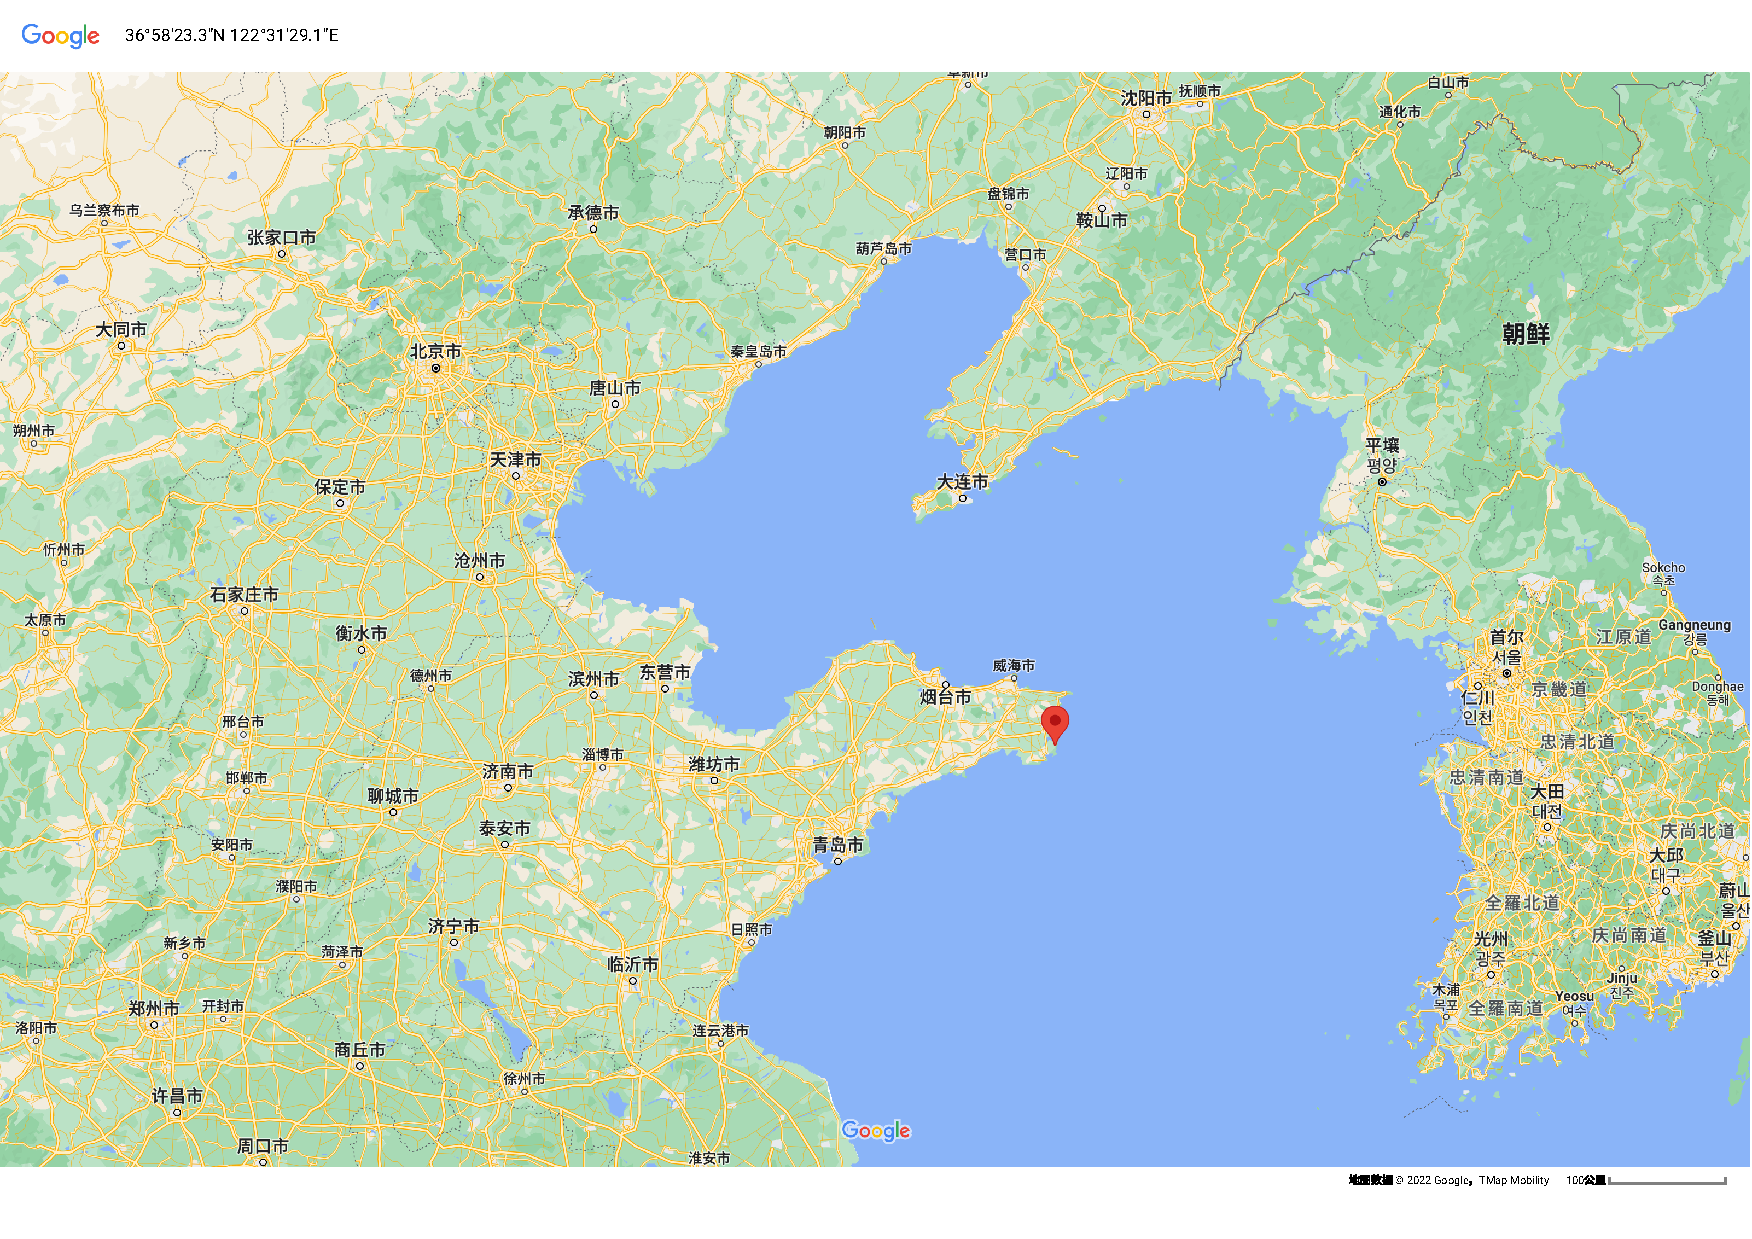
\includepdf[width=0.7\linewidth]{figures/shidaowan.pdf}
    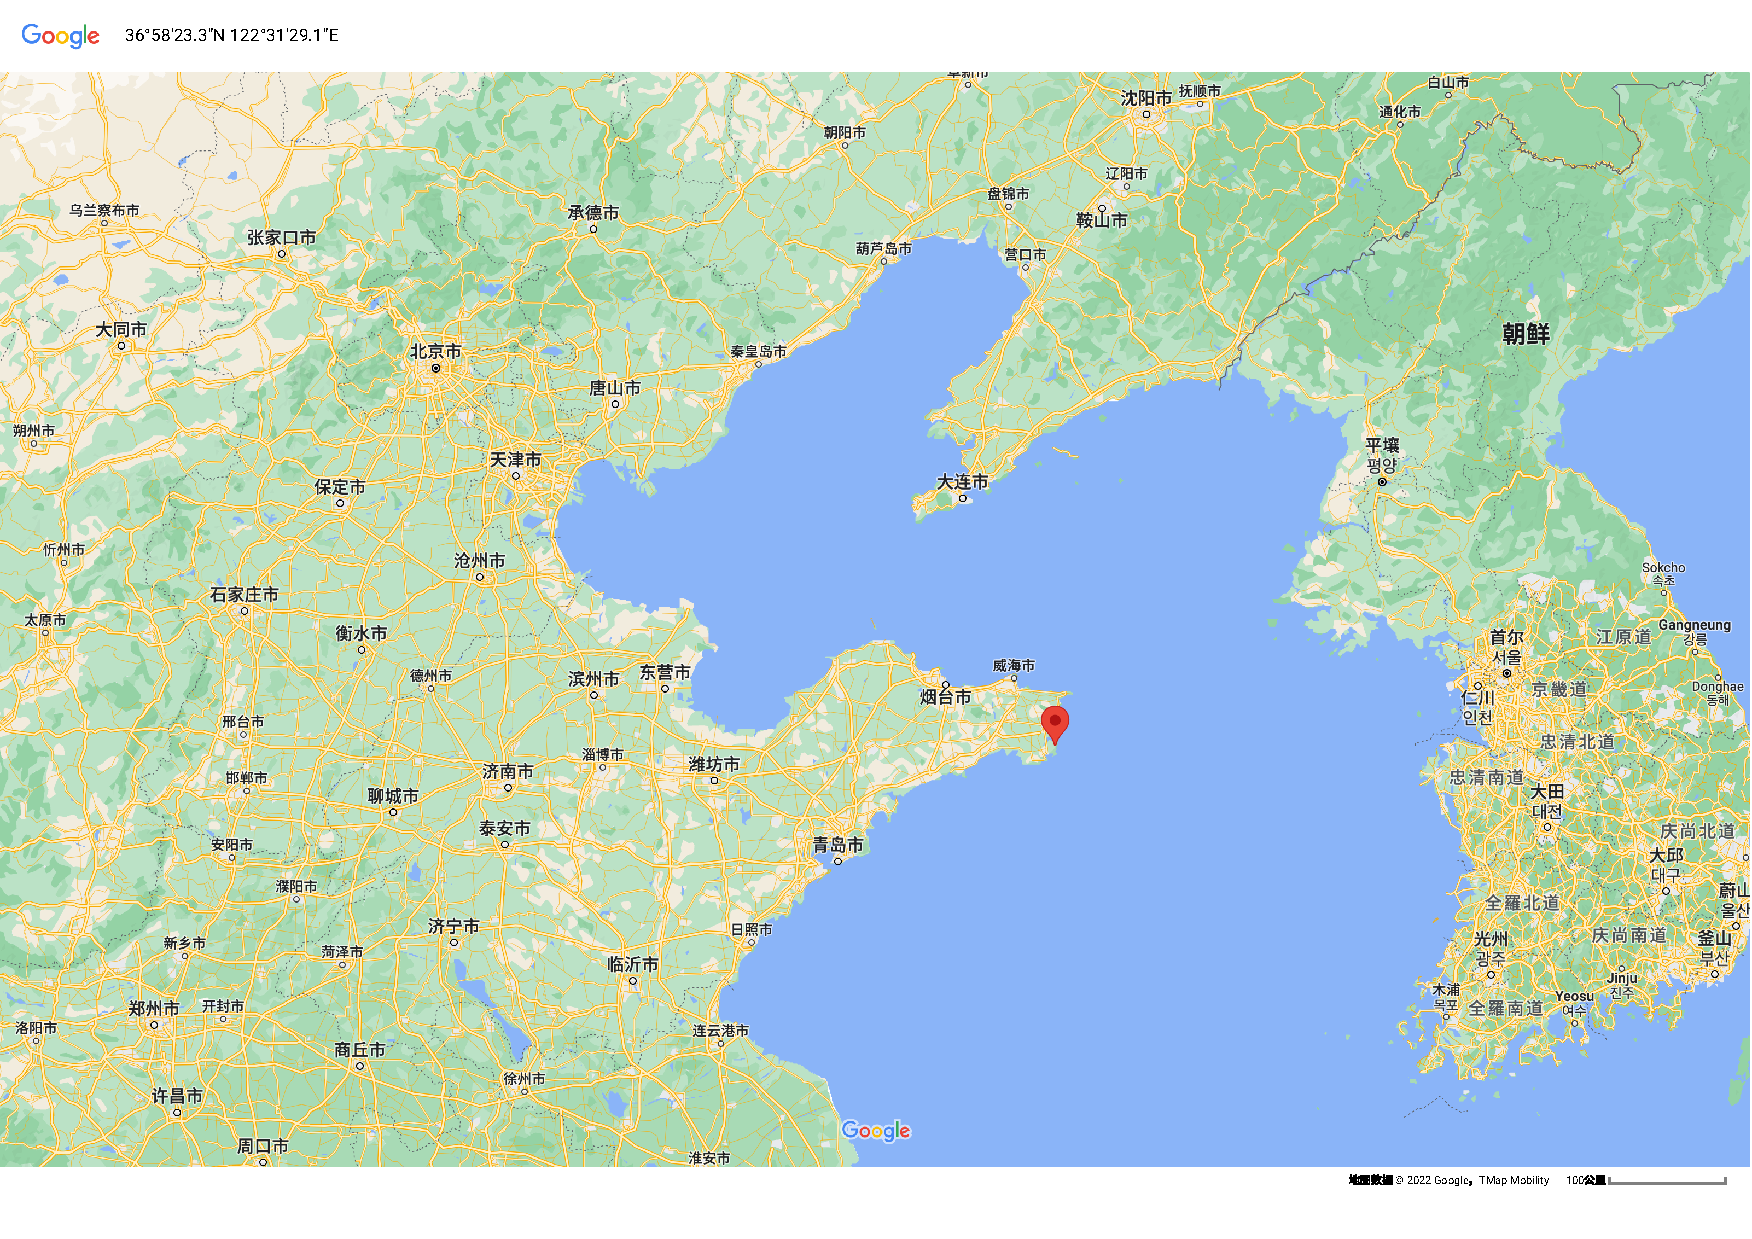
\includegraphics[width=1.0\linewidth]{figures/shidaowan.pdf}
    \caption{\label{fig:shidaowan} 计划中的LXeTPC实验的选址位置。图片来源:Google Maps.\cite{shidaowan_googlemap_220524}。}
\end{figure}



\section{LXeTPC探测CE$\nu$NS信号}
\label{sec:lxe_signal}

\section{HPGe探测器的CE$\nu$NS信号}

% !TeX root = ../main.tex

\chapter{地面运行的LXeTPC本底研究}
\label{sec:backgrounds}

为了定量地描述实验对某些物理参数的灵敏度,我们需要对实验本底进行估计。
本章使用蒙特卡洛方法(Monte Carlo method),估计两类实验中的主要本底:$\mu$子本底和材料放射性本底,
以及信号筛选条件对两类本底的压低能力。

\section{模拟框架}

Geant4 是辐射探测和粒子物理领域常用的以C++为基础的蒙特卡洛模拟软件包\cite{agostinelli_geant4simulation_2003,allison_geant4_2006,allison_recent_2016}。
PandaX合作组基于Geant4开发了BambooMC软件包用于PandaX实验中的探测器模拟\cite{chen_bamboomc_2021}。
BambooMC具有较强的可拓展性,本文中使用基于BambooMC开发的软件包RelicsSim对地表附近探测器$\mu$事件和材料本底进行模拟。
所用几何如图\ref{fig:relics_g4}所示,结构遵循\ref{fig:relics_geo}的设计。

\begin{figure}
  \begin{subfigure}{.5\textwidth}
    \centering
    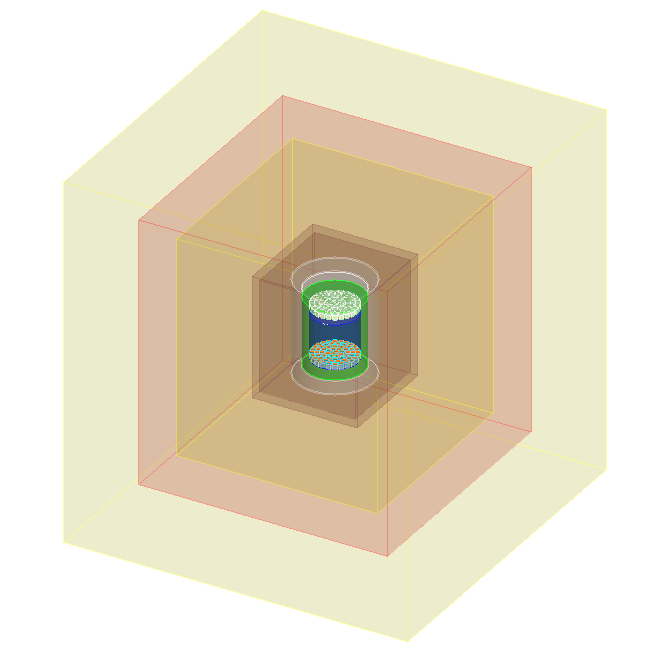
\includegraphics[width=1.0\linewidth]{figures/relics_outer.png}
    \caption{\label{fig:relics_outer} LXeTPC屏蔽体几何}
  \end{subfigure}
  \begin{subfigure}{.5\textwidth}
    \centering
    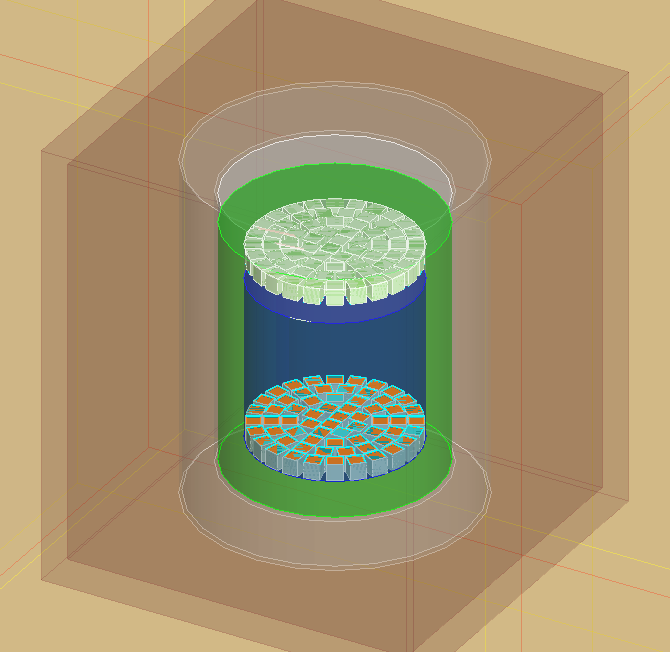
\includegraphics[width=1.0\linewidth]{figures/relics_inner.png}
    \caption{\label{fig:relics_inner} LXeTPC中心探测器几何}
  \end{subfigure}
  \caption{\label{fig:relics_g4} RelicsSim中屏蔽体和探测器几何探测器,绿色体积为液氙4$\pi$反符合探测器,蓝色体积为中心主探测器。}
\end{figure}

探测器基本参数列在表\ref{tab:relics_material}中。

\begin{table}
  \centering
  \caption{LXeTPC几何参数}
  \begin{tabular}{cccc}
    \toprule
    名称 & 几何体 & 参数 & 材料 \\
    \midrule
    外聚乙烯屏蔽体 & 空心长方体 & $216\times216\times226\si{cm^3}$ & 高密度聚乙烯 \\
    铅屏蔽体 & 空心长方体 & $156\times156\times166\si{cm^3}$ & 铅 \\
    内聚乙烯屏蔽体 & 空心长方体 & $126\times126\times136\si{cm^3}$ & 高密度聚乙烯 \\
    铜屏蔽体 & 空心长方体 & $66\times66\times76\si{cm^3}$ & 铅 \\
    空气层 & 空心长方体 & $60\times60\times70\si{cm^3}$ & 空气 \\
    外不锈钢罐体 & 空心圆柱体 & 厚度$0.5\si{cm}$,高$59\si{cm}$,直径$48\si{cm}$ & 不锈钢 \\
    真空隔热层 & 空心圆柱体 & 厚度$5\si{cm}$,高$58\si{cm}$,直径$47\si{cm}$ & 真空 \\
    内不锈钢罐体 & 空心圆柱体 & 厚度$0.5\si{cm}$,高$48\si{cm}$,直径$37\si{cm}$ & 不锈钢 \\
    外层气态氙 & 圆柱体 & 高$5\si{cm}$,直径$36\si{cm}$ & 气态氙 \\
    液氙反符合层 & 空心圆柱体 & 厚度$4\si{cm}$,高$42\si{cm}$,直径$36\si{cm}$ & 液态氙 \\
    内层气态氙 & 圆柱体 & 高$6\si{cm}$,直径$28\si{cm}$ & 气态氙 \\
    液氙主探测器 & 圆柱体 & 高$28\si{cm}$,直径$28\si{cm}$ & 液态氙 \\
    \bottomrule
  \end{tabular}
  \label{tab:relics_material}
\end{table}

液氙主探测器上下分别有64个1英寸光电倍增管:日本滨松R8520,共128个。光电倍增管的几何如图\ref{fig:pmt_geo}。

\begin{figure}
  \begin{subfigure}{.52\textwidth}
    \centering
    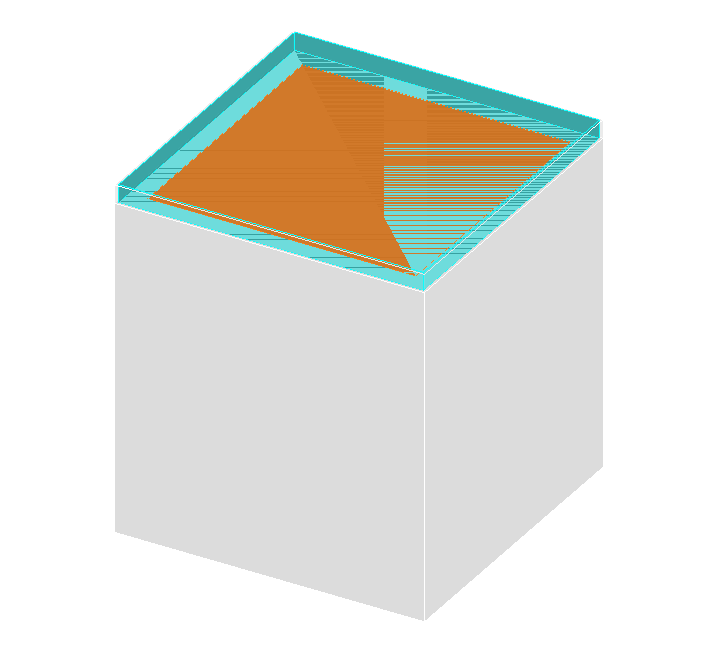
\includegraphics[width=1.0\linewidth]{figures/pmt_geo.png}
    \caption{\label{fig:pmt_g4} R8520在Geant4中的几何}
  \end{subfigure}
  \begin{subfigure}{.48\textwidth}
    \centering
    \includesvg[width=1.0\linewidth]{figures/topPMTs.svg}
    \caption{\label{fig:pmt_layout} PMT在探测器$(x,y)$平面上的排布}
  \end{subfigure}
  \caption{\label{fig:pmt_geo} 光电倍增管R8520的几何和在探测器$(x,y)$平面上的排布。
  蓝色透明几何为石英窗;橙色几何为光阴极(photocathode);灰色部分是外壳(casing),材质为SAE 304不锈钢。
  排布保证了轴向对称性,可能对未来的位置重建有利。}
\end{figure}

PMT石英窗上富集的${}^{40}\mathrm{K}$和${}^{137}\mathrm{Cs}$可能成为主要的本底来源,具体内容将在第\ref{sec:pmt_background}章中讨论。

\section{本底事件的筛选与压低}

本底事件经常与信号有不同的性质以及测量结果。
我们可以通过选取某些具有区分能力(discrimination power)的性质,在其值域中定义选取信号并进行物理分析的区间,
在尽可能少地损失信号的条件下,去除尽可能多的本底。

对于$\mu$子本底,其可能强烈地在液氙反符合层中沉积能量,可以用反符合层对$\mu$子的标记将其本底压低。
考虑到一个物理事件的时间窗约为$200\mu s$,$\mu$子和中子将可能有足够多的时间在主探测器中多次沉积能量,
而中微子几乎只可能与探测器发生单次散射(single scatter, SS),
所以我们可以通过筛选并去除一个事件窗内有多次散射(multiple scatter, MS)的事件,对这类本底进行压低。
最后,若一个主探测器中的核反冲事件同时伴随着一个主探测器中的电子反冲事件,则这个核反冲事件有较大可能是$\mu$子引起的而不是中微子。

材料的$\beta$和$\gamma$放射性在中心探测器边缘单位体积沉积的能量比探测器中心多,所以一定程度地舍弃某些本底过高的区域,
对物理信号的搜索是有利的,选取的本底较低的区域定义为灵敏体积(fiducial volume)。
同时材料本底,有一定概率产生多次散射,如$\gamma$的康普顿散射事件,也可以通过判断是否有多次散射来去除这类本底。

所有与能量相关的筛选条件(或阈值)均需要通过详尽严格的信号模拟来确定;
灵敏体积的选取和设置也需要综合考虑物理信号和本底的空间分布。本文仅根据经验,设置粗略的信号筛选条件,
考察在这些条件下信号和本底的事例率以及相应的实验灵敏度。
针对核反冲本底和电子反冲本底,信号筛选条件列于表\ref{tab:cuts},只有满足表中所有条件的事件才被纳入物理分析。

\begin{table}
  \centering
  \caption{针对核反冲和电子反冲本底的信号筛选条件}
  \begin{tabular}{cc}
    \toprule
    名称 & 条件 \\
    \midrule
    液氙反符合(LXe veto) & 反符合层中最大的电子(核)反冲不大于$100$($500$)$\si{keV}$ \\
    NR单次散射(ER SS cut) & 主探测器中第二大的NR能量不大于最大NR能量的5\% \\
    ER单次散射(NR SS cut) & 主探测器中第二大的ER能量不大于$1\si{keV}$ \\
    NR的ER标记(ER tagging) & 主探测器中与NR事件同时发生的ER不大于$10\si{keV}$ \\
    灵敏体积(FV cut) & 气液交界面以下$0.5\si{cm}$到$24.5\si{cm}$,半径$12\si{cm}$的圆柱 \\
    \bottomrule
  \end{tabular}
  \label{tab:cuts}
\end{table}

反符合层中没有漂移电场,只有光信号,我们将在反符合层中设置PMT来探测这他们。
由于核反冲信号的淬灭效应,相同能量的核反冲和电子反冲产生的光子数不同,取淬灭因子(quenching factor)为0.2,
则将反符合层的核反冲阈值设置为电子反冲的$1/0.2=5$倍。

灵敏体积为高$24\si{cm}$,半径为$12\si{cm}$的圆柱,其中液氙总质量约为$30.5\si{kg}$。在S2-Only分析中,不引入$\mathrm{S1}$,
事件将没有电子漂移距离$z$信息,但我们让然可以通过$\mathrm{S2}$波形的事件分布一定程度上判断事件发生的纵向位置,
所以这里对S2-Only和S1-S2分析设置了相同的灵敏体积。

\section{$\mu$子本底}

地面附近运行的LXeTPC将会经受原生宇宙线和次生宇宙线的轰击。
来自外部空间的宇宙线成分以高能质子为主,在穿越地球大气层的过程中与大气分子发生簇射反应,产生大量次级粒子,
主要包括质子、$\mu$子、电子、中子、$\gamma$光子等。宇宙线粒子通量与大气层深度有关,如图\ref{fig:vertical_flux}。

\begin{figure}
    \centering
    \includesvg[width=0.7\linewidth]{figures/vertical_flux.svg}
    \caption{\label{fig:vertical_flux} 宇宙线中不同粒子通量与大气深度的关系\cite{olive_review_2016}。
    $\mu$子和中微子是地面附近通量最高的两种粒子,中微子较少与物质发生相互作用,$\mu$子成为实验中的主要本底。}
\end{figure}

$\mu$子是带电粒子,穿透能力较强。$\mu$子穿越物质的过程中通过电磁相互作用减速,产生电离,
高能($10\si{GeV}$以上)$\mu$子在物质中的能损$-\mathrm{d}E/\mathrm{d}x$大约为$2\si{MeV\cdot cm^{-1}}$。
考虑相对论时间膨胀效应,$\mu$子在物质中能够穿越较长距离。$\mu$子还有可能被原子核俘获,
使靶原子核序数减1,同时放出1个或多个中子。这些中子将是探测器中核反冲本底的主要来源。

利用$\mu$子持续产生电离的特点,可以在探测器外围部署$\mu$子反符合探测器,
当$\mu$子同时在反符合探测器和主探测器产生信号且符合一定条件时时,通过硬件触发或软件筛选,
可以将主探测器中事件标记为$\mu$子事件以区分信号的本底。但物理信号如CE$\nu$NS也有一定几率发生在$\mu$子穿越探测器时,
这时对$\mu$子事件的标记会使物理信号的探测效率降低,等效为曝光量(exposure)的损失,这种效应必须考虑到统计推断中,
否则将高估探测器中产生的信号。

地面附近的$\mu$子分布可以用Gaisser公式或Shukla公式描述。T.K.Gaisser在忽略地球曲率的情况下,
给出了$\mu$子通量随$\mu$子能量$E_\mu$和天顶角(zenith angle)$\theta$的分布。天顶角为入射粒子与地面法线间的夹角\cite{gaisser_cosmic_2016}。

\begin{align}
    \label{eq:gaisser}
    \frac{\mathrm{d}N_\mu}{\mathrm{d}E_\mu\mathrm{d}\Omega} &\approx 
    1400E_\mu^{-2.7}/\left(\si{m^2\cdot s\cdot GeV\cdot sr}\right)\left(\frac{1}{1+\frac{1.1E_\mu\cos\theta}{\epsilon_\pi}}+\frac{0.054}{1+\frac{1.1E_\mu\cos\theta}{\epsilon_\kappa}}\right)
\end{align}

其中$\epsilon_\pi\approx115\si{GeV},\epsilon_\kappa\approx850\si{GeV}$。
Gaisser公式只在高能区间($E_\mu>(100/\cos\theta)\si{GeV}$)适用。

P.Shukla等人在考虑地球曲率的条件下给出了类似的分布\cite{shukla_energy_2018},如式\ref{eq:shukla}:

\begin{align}
    \label{eq:shukla}
    I\left(E_\mu,\theta\right) &= I_0 N\left(E_0+E_\nu\right)^{-n}\left(1 + \frac{E_\mu}{\epsilon_\mu}\right)^{-1}D(\theta)^{-(n-1)} \\
    D(\theta) &= \sqrt{\frac{R^2}{d^2}\cos^2\theta+2\frac{R}{d}+1}-\frac{R}{d}\cos\theta
\end{align}

其中$I_0$为绝对流强,$N$为归一化参数,$n$为天顶角分布的幂次,$\epsilon_\mu,\frac{R}{d}$为经验公式中的自由参数。
使用不同地点测量得到的$\mu$子分布可以拟合得到不同结果,这里我们使用Shukla通过日本筑波市附近的测量数据得到的拟合结果,具体参数见表\ref{tab:shukla}。
Shukla公式在低能区域和高能区域都与数据符合得较好。

\begin{table}
  \centering
  \caption{描述$\mu$子分布的Shukla公式采用的参数列表}
  \begin{tabular}{cc}
    \toprule
    符号 & 取值 \\
    \midrule
    $I_0$ & $70.7\si{m^{-2}\cdot s^{-1}\cdot sr^{-1}}$ \\
    $n$ & 3.01 \\
    $E_0$ & $4.19\si{GeV}$ \\
    $\epsilon_\mu$ & $854\si{GeV}$ \\
    $R/d$ & $174$ \\
    \bottomrule
  \end{tabular}
  \label{tab:shukla}
\end{table}

式\ref{eq:shukla}中天顶角$\theta$相关的项可以从$E_\mu$中解耦合,$\theta$和$E_\mu$的分布如图\ref{fig:shukla_distribution}。

\begin{figure}
    \centering
    \includesvg[width=1.0\linewidth]{figures/shukla_distribution.svg}
    \caption{\label{fig:shukla_distribution} Shukla公式中$\theta$和$E_\mu$的分布,$\theta$主要集中在夹角较小的区域,
    因为天顶角更大的$\mu$子与大气层中物质的相互作用路程更长,损失更多;$E_\mu$的分布主要集中在低能部分。}
\end{figure}

对Shukla公式进行积分,可以得到海平面附近全能谱$\mu$子通量约为$150\si{m^{-2}\cdot s^{-1}}$。

到达地面附近的$\mu$子包含了$\mu^-$和$\mu^+$。
CMS于2010年测量得到了地表附近的$\mu$子电荷比(charge ratio, $I_{\mu^+}/I_{\mu^-}$)约为$1.2766\pm0.0045$\cite{the_cms_collaboration_measurement_2010}。
$\mu$子电荷比在$\mu$子动量小于$100\si{GeV/c}$时与能量几乎无关,且在更高动量的区域略增大。
考虑到第\ref{sec:muon_nr}节中讨论的$\mu$子核反冲本底主要由较低能量的$\mu^-$贡献,更高的电荷比意味着更低的核反冲本底,本文保守地使用不随能量变化的电荷比。

模拟中将从屏蔽体外部一个足够的水平平面上均匀取点作为$\mu$子的入射位置,通过Shukla公式对$\mu$子的入射角和能量进行采样,
模拟几何如图\ref{fig:muon_inject}。

\begin{figure}
  \centering
  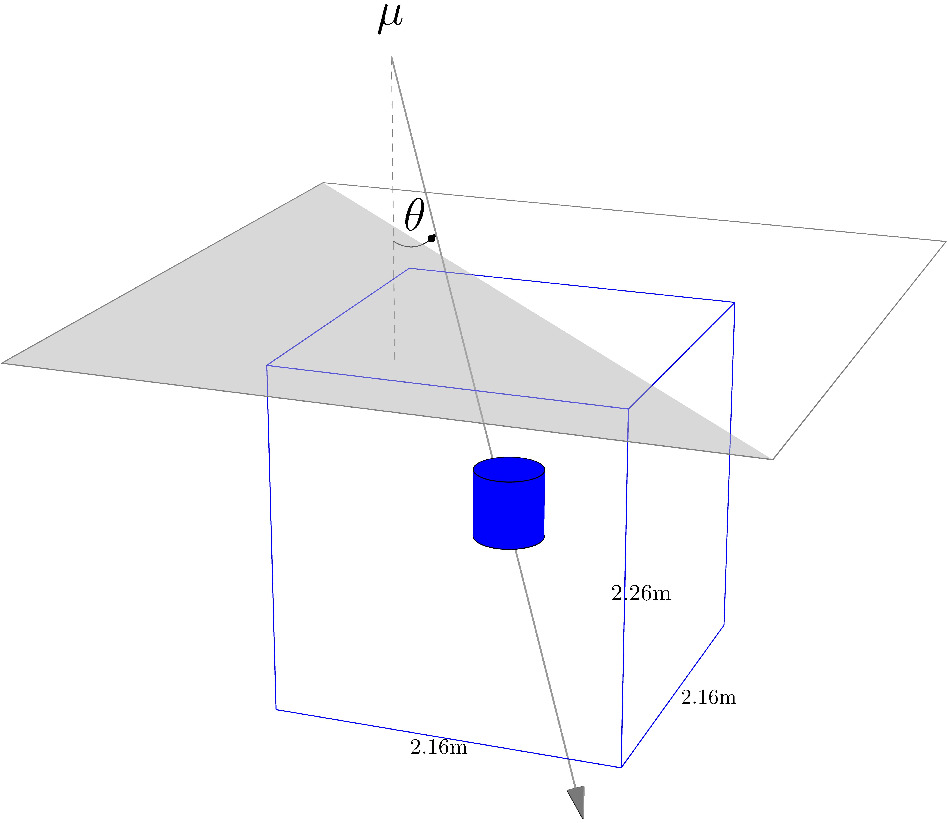
\includegraphics[width=0.6\linewidth]{figures/muon_inject.pdf}
  \caption{\label{fig:muon_inject} $\mu$子入射屏蔽体和探测器的示意图。
  最顶部平面为$\mu$子初始位置,蓝色圆柱体为液氙探测器。}
\end{figure}

Geant4模拟中设置中心探测器和液氙反符合屏蔽层为灵敏探测器,并记录两种灵敏探测器中的能量沉积。
因液氙中相近时间且相近空间位置的能量沉积并不能被有效区分,
得到模拟结果后将使用聚类算法DBSCAN(Density-Based Spatial Clustering of Applications with Noise)\cite{ester_density-based_1996,schubert_dbscan_2017}合并临近时空中的能量沉积。

本文中假设$\mu$子反符合探测器的探测效率为99\%,且不随$\mu$子能量变化,
即假设只有1\%的$\mu$子事件的能量沉积不能被$\mu$子反符合探测器标记并最终形成被记录的本底。

\subsection{核反冲本底}
\label{sec:muon_nr}

$\mu$子主要通过两种方式产生核反冲。高能$\mu$子可以直接与原子核发生库伦散射使原子核获得动能;
低能$\mu$子有跟高的概率被原子核俘获,之后放出一个或几个中子。图\ref{fig:muon_nr}列出了$\mu$子引起核反冲的总能谱。

\begin{figure}
  \centering
  \includesvg[width=0.9\linewidth]{figures/muon_nr.svg}
  \caption{\label{fig:muon_nr} $\mu$子引起的核反冲能谱。
  其中按顺序施加了灵敏体积、液氙反符合、对核反冲的电子反冲标记、核反冲单次散射等筛选条件。}
\end{figure}

液氙反符合对$\mu$子核反冲的压低能力在我们关心的能区$[0.1,1]\si{keV}$最强,
因为低能中子产生多次散射的概率不高,NR SS cut的压低能力并不显著,图中只有高能部分的NR被其显著压低。
在施加筛选条件之后,$[0.1,1]\si{keV}$中的事例率为$0.30\left(\si{kg}\cdot\si{day}\right)^{-1}$,空间分布如图\ref{fig:muon_nr_xyzr}。

\begin{figure}
  \centering
  \includesvg[width=1.0\linewidth]{figures/muon_nr_xyzr.svg}
  \caption{\label{fig:muon_nr_xyzr} $\mu$子引起的核反冲经过筛选条件压低后的空间分布,
  在$(x,y)$和$(r^2,z)$投影上都比较均匀。}
\end{figure}

\subsection{电子反冲本底}

$\mu$子带电,$\mu$子事件的电子反冲本底主要由$\mu$子在物质中的直接电离引起。如图\ref{fig:muon_er}。

\begin{figure}
  \centering
  \includesvg[width=1.0\linewidth]{figures/muon_er.svg}
  \caption{\label{fig:muon_er} $\mu$子引起的电子反冲能谱,左图:全区能谱,右图:$[0, 100]\si{keV}$能区能谱。
  其中按顺序施加了灵敏体积、液氙反符合、电子反冲单次散射等筛选条件。}
\end{figure}

对于高能$\mu$致电子反冲,液氙反符合的效果非常明显,在施加该条件后,几乎所有$5\si{MeV}$以上的电子反冲事件都会被排除。
要求电子反冲单次散射也会将本底压低近1个量级。
以致\ref{fig:muon_er}右图能谱的形状可能是低能区域模拟事件统计量的涨落所致,也可能是$\mu$子对物质原子核激发产生的特征$\gamma$射线的能谱,具体原因有待考察。

\begin{figure}
  \centering
  \includesvg[width=1.0\linewidth]{figures/muon_er_xyzr.svg}
  \caption{\label{fig:muon_er_xyzr} $\mu$子引起的电子反冲经过筛选条件压低后的空间分布,在探测器上部分布略集中。}
\end{figure}

表\ref{tab:cuts_muon_remain}列出了几种筛选条件后的$\mu$子核反冲在$[0.1,1]\si{keV}$能区和电子反冲在的$[0,100]\si{keV}$能区剩余事例率,误差棒来自模拟事例个数的统计误差。

\begin{table}
  \centering
  \caption{$\mu$子引起的$[0.1,1]\si{keV}$内核反冲和$[0,100]\si{keV}$内电子反冲的本底剩余事例率}
  \begin{tabular}{ccc}
    \toprule
    筛选条件 & $T_\mathrm{nr}\left(10^{-2}\left(\si{kg}\cdot\si{day}\right)^{-1}\right)$ & $T_\mathrm{er}\left(10^{-3}\left(\si{kg}\cdot\si{keV}\cdot\si{day}\right)^{-1}\right)$ \\
    \midrule
    无筛选条件 & $122.8_{-10.1}^{+11.0}$ & $44.9_{-2.0}^{+2.1}$ \\
    灵敏体积(FV cut) & $70.6_{-7.6}^{+8.5}$ & $12.2_{-1.0}^{+1.1}$ \\
    液氙反符合(LXe veto) & $23.8_{-4.2}^{+5.1}$ & $6.6_{-0.7}^{+0.8}$ \\
    NR的ER标记(ER tagging) & $21.1_{-3.9}^{+4.8}$ & - \\
    NR单次散射(NR SS cut) & $21.1_{-3.9}^{+4.8}$ & - \\
    ER单次散射(ER SS cut) & - & $4.0_{-0.6}^{+0.7}$ \\
    \bottomrule
  \end{tabular}
  \label{tab:cuts_muon_remain}
\end{table}

\section{材料本底}

相比于$\mu$子本底,材料本底是地面实验和地下实验都需要处理的本底。
材料本底主要来自屏蔽体、罐体、光电倍增管、整形环、聚四氟乙烯反射板、以及液氙等。
本文主要模拟来自屏蔽体、光电倍增管和液氙的放射性本底。

因一半放射性同位素含量与材料有关而与材料所处空间位置基本无关,BambooMC设计了\verb|Confine Generator|用于模拟某种材料放射性。
其工作原理如下:首先指定需要进行模拟的材料,然后随机在足够大的空间中均匀采样,通过设计的几何关系判断采样点对应的几何体的材料是否为预先指定的,
若是,则放置放射性核素的原子(或离子);若不是,则继续在空间中撒点直到选取到指定的材料为止。这种模拟方式不需要精确描述放射源的初始位置,较简便,
同时也默认了所有材料放射源在材料中均匀分布。

屏蔽体和罐体的材料主要为金属。金属矿石与长半衰期的原生放射性核素共生,
如${}^{238}\mathrm{U},{}^{232}\mathrm{Th},{}^{40}\mathrm{K}$等。
PMT石英窗(主要成分为$\mathrm{Si}\mathrm{O}_2$)因为$\mathrm{Si}$与碱金属元素的亲和性,也含有一定量的${}^{40}\mathrm{K}$元素。
这些核素的半衰期非常长,如${}^{238}\mathrm{U}$的半衰期为45亿年。
如此长的半衰期使得,在矿石中这些核素与其衰变链上的子核将建立稳定平衡(secular equilibrium),具体表现为母核核素与子核核素的放射性活度相等。
这对我们计算核素长衰变链上的放射性活度提供了便利。
然而事实上对矿石的开采冶炼和一些其他过程可能会破坏稳定平衡,导致母核与子核核素的活度不等,此时为了估计材料放射性,就需要对进行实地测量,
并以实地测量的结果作为蒙特卡洛的输入量。本文中假定稳定平衡不被破坏,即将长半衰期核素的活度作为全衰变链上子核的活度,
如认为${}^{238}\mathrm{U}$与其链上的${}^{226}\mathrm{Ra}$活度相等。

金属中还可能含有${}^{60}\mathrm{Co}$等人工放射性核素和${}^{3}\mathrm{H}$等宇生放射性核素,在模拟中也将一并考虑。

BambooMC提供了\verb|DecayChainSplitting|功能用于模拟衰变链上的核素。考虑到探测器的时间窗约为$200\mu s$,
则衰变链上的较长半衰期核素如${}^{226}\mathrm{Ra}$($T_{1/2}=1602y$)几乎可能与其母核在同一个时间窗内衰变。在模拟中,我们可以将衰变链通过判断核素半衰期长度的方式分解。
首先设置一个阈值,如$200\mu s$,对于任何半衰期长于阈值的核素,我们都将其作为一个新的模拟事件的母核对待,
同时新事件的时间也会归零,这样很大程度上与实际情况是符合的。这种操作减少了遍历每一种衰变链上核素的工作量。

\subsection{光电倍增管本底}
\label{sec:pmt_background}

光电倍增管(PMT)上的本底主要有石英窗上的${}^{40}\mathrm{K},{}^{137}\mathrm{Cs},{}^{238}\mathrm{U}$和金属外壳上的${}^{238}\mathrm{U},{}^{232}\mathrm{Th}$等,即这些核素的子核。
模拟中的PMT结构见图\ref{fig:pmt_geo}。放射性核素的具体含量见表\ref{tab:pmt_radio},数据来自XENON100的电子反冲本底研究\cite{xenon100_collaboration_study_2013}。

\begin{table}
  \centering
  \caption{PMT上每部分结构放射性同位素比活度,单位均为$\si{mBq\cdot kg^{-1}}$}
  \begin{tabular}{ccc}
    \toprule
    核素 & PMT石英窗 & PMT外壳 \\
    \midrule
    ${}^{238}\mathrm{U}$ & 0.14 & 0.16 \\
    ${}^{232}\mathrm{Th}$ & 0.17 & 0.07 \\
    ${}^{60}\mathrm{Co}$ & 0.62 & 0.01 \\
    ${}^{40}\mathrm{K}$ & 11.1 & 0.16 \\
    ${}^{137}\mathrm{Cs}$ & 0.79 & 0 \\
    \bottomrule
  \end{tabular}
  \label{tab:pmt_radio}
\end{table}

模拟中PMT的石英窗质量为$2\si{g}$,外壳质量为$13.6\si{g}$。

\subsection{屏蔽体材料本底}

屏蔽体和罐体材料中的本底含量如表\ref{tab:shield_radio}。

\begin{table}
  \centering
  \caption{屏蔽体和罐体组件中放射性同位素比活度,单位均为$\si{mBq\cdot kg^{-1}}$}
  \begin{tabular}{ccccc}
    \toprule
    核素 & 聚乙烯屏蔽层 & 铅屏蔽层 & 铜屏蔽层 & 不锈钢罐体 \\
    \midrule
    ${}^{238}\mathrm{U}$ & 0.23 & 0.92 & 0.08 & 1.8 \\
    ${}^{232}\mathrm{Th}$ & 0.09 & 0.72 & 0.01 & 1.9 \\
    ${}^{60}\mathrm{Co}$ & 0 & 0.12 & 0.04 & 5.4 \\
    ${}^{40}\mathrm{K}$ & 0.68 & 0.01 & 0.03 & 9 \\
    ${}^{210}\mathrm{Pb}$ & 0 & $5.14\times10^5$ & 0 & 0 \\
    \bottomrule
  \end{tabular}
  \label{tab:shield_radio}
\end{table}

\subsection{液氙中惰性元素本底}

本文中主要考虑的液氙中惰性元素本底为${}^{222}\mathrm{Rn}$和${}^{85}\mathrm{Kr}$。

${}^{222}\mathrm{Rn}$在${}^{238}\mathrm{U}$的衰变链中产生,探测器材料会持续放出${}^{222}\mathrm{Rn}$。
考虑到${}^{222}\mathrm{Rn}$半衰期为$3.8d$,其和其子核将在液氙体积中均匀地衰变。
本文中假定其比活度为$60\si{mBq\cdot kg^{-1}}$。
${}^{222}\mathrm{Rn}$衰变链上的${}^{210}\mathrm{Pb}$半衰期为$22.4y$,相比于探测器运行时间,
${}^{210}\mathrm{Pb}$对放射性的贡献可以忽略,其后续所有衰变的放射性也将不考虑到模拟结果中。

自然界的$\mathrm{Kr}$元素中含有痕量的${}^{85}\mathrm{Kr}$(半衰期$T_{1/2}=10.76y$)。
其$\beta$衰变能谱中最大能量为$685\si{keV}$,使其在低能分析中,成为不可忽略的重要本底。
${}^{85}\mathrm{Kr}$的丰度为${}^{85}\mathrm{Kr}/{}^\mathrm{nat}\mathrm{Kr}=(1.7\pm0.3)\times 10^{-11}$。
本文中假定${}^\mathrm{nat}\mathrm{Kr}$在液氙中的含量为$6\mathrm{nat}{}^{85}\mathrm{Kr}/\mathrm{Xe}$,且${}^{85}\mathrm{Kr}$活度不随着时间变化。

将所有材料放射性的电子反冲本底叠加,得到汇总,如图\ref{fig:muon_er}。

\begin{figure}
  \centering
  \includesvg[width=1.0\linewidth]{figures/material_er.svg}
  \caption{\label{fig:material_er} 材料放射性电子反冲本底汇总。左图:全区能谱,右图:$[0, 100]\si{keV}$能区能谱。
  其中按顺序施加了灵敏体积、液氙反符合、电子反冲单次散射等筛选条件。}
\end{figure}

灵敏体积 cut 对电子反冲本底的压低效果很强,这主要是因为$\mathrm{Xe}$的辐射屏蔽效果很强,PMT放射性大多集中在TPC的阴极以下及液氙上表面;
且不锈钢罐体的主要放射性集中靠近罐体的区域。电子反冲单词散射对较高能的本底压低效果很强,因为几百$\si{keV}$的$\gamma$光子更容易产生多次散射效应。

低能区域($[0, 100]\si{keV}$)的能谱较平坦,在施加筛选条件后主要剩余本底来自于${}^{85}\mathrm{Kr}$和PMT,${}^{222}\mathrm{Rn}$的贡献在$1\times10^{-3}\si{kg}\cdot\si{keV}\cdot\si{day}$以下。

\begin{figure}
  \centering
  \includesvg[width=1.0\linewidth]{figures/material_er_xyzr.svg}
  \caption{\label{fig:material_er_xyzr} 材料放射性电子反冲本底经过筛选条件压低后的空间分布,
  略集中在灵敏体积边缘。}
\end{figure}

表\ref{tab:cuts_material_remain}列出了几种筛选条件后的材料放射性电子反冲本底在$[0,100]\si{keV}$能区剩余事例率,误差棒来自模拟事例个数的统计误差。

\begin{table}
  \centering
  \caption{材料放射性引起的$[0.1,1]\si{keV}$内核反冲和$[0,100]\si{keV}$内电子反冲的本底剩余事例率}
  \begin{tabular}{ccc}
    \toprule
    筛选条件 & $T_\mathrm{er}\left(10^{-3}\left(\si{kg}\cdot\si{keV}\cdot\si{day}\right)^{-1}\right)$ \\
    \midrule
    无筛选条件 & $1821.0_{-4.1}^{+4.1}$ \\
    灵敏体积(FV cut) & $54.0_{-0.5}^{+0.5}$ \\
    液氙反符合(LXe veto) & $23.5_{-0.2}^{+0.2}$ \\
    NR的ER标记(ER tagging) & $18.8_{-0.2}^{+0.2}$ \\
    \bottomrule
  \end{tabular}
  \label{tab:cuts_material_remain}
\end{table}

图\ref{fig:all_event_rate}是两种本底和信号的汇总,因核反冲信号的淬灭效应,取淬灭因子为0.2,
将核反冲能量$T_\mathrm{nr}$乘淬灭因子转化后与电子反冲能量进行比较。

\begin{figure}
  \centering
  \includesvg[width=0.8\linewidth]{figures/all_event_rate.svg}
  \caption{\label{fig:all_event_rate} $\mu$子与材料的核反冲本底和电子反冲本底汇总,蓝色阴影为进行物理搜索的主要能区。}
\end{figure}

% !TeX root = ../main.tex

\chapter{LXeTPC与HPGe探测器对CE$\nu$NS探测的灵敏度}

\section{中微子超标准模型有效相互作用测量}

\section{低动量转移下的弱混合角测量}

\section{低能核反冲的液氙光电产额测量}

% !TeX root = ../main.tex

\chapter{总结与展望}

本文建立了LXeTPC测量反应堆中微子CE$\nu$NS信号的本底模拟框架和灵敏度预测框架。

若可以控制地面附近的本底,尤其是$\mu$子引起的核反冲本底,
$30\si{kg\cdot y}$曝光量的LXeTPC对中微子超标准模型有效相互作用参数的灵敏度将达到世界领先,
对弱混合角的测量也将填补实验空白。

研究中建立的模拟框架可以用于优化探测器几何设计和本底控制。

研究中对信号相应进行了一定量的近似,如TPC光收集效率和$\mathrm{S2}$增益的计算中未考虑探测器几何效应,
对4个及以上的漂移电子采用了100\%的探测效率。同时未完全考虑探测器的几何细节如聚四氟乙烯反射板、整形环等。
在未来的研究中将建立完整的探测器几何模型进行光学模拟和电场模拟以确定几何效应。

HPGe探测器灵敏度计算中未考虑地面中子本底的水平,应针对$\mu$子设计相应的屏蔽体结构,建立类似的模拟框架。

本底计算中使用了简单的长期平衡假设,在探测器实际运行中将实际测量材料的俄各种放射性含量后进行模拟。
模拟后使用的能量沉积聚类算法的计算效率有限,$\mu$子模拟个数不足够高以消除模拟中的统计误差。

$\mu$子反符合探测器将引入曝光量损失,$\mu$子沉积能量引起的偶然符合等本底也会引入曝光量损失,这也是未来分析中需要考虑的。



% 其他部分
\backmatter

% 插图和附表清单
% 本科生的插图索引和表格索引需要移至正文之后、参考文献前
% \listoffiguresandtables  % 插图和附表清单(仅限研究生)
\listoffigures           % 插图清单
\listoftables            % 附表清单

% 参考文献
\bibliography{ref/refs}  % 参考文献使用 BibTeX 编译
% \printbibliography       % 参考文献使用 BibLaTeX 编译

% 致谢
% !TeX root = ../thuthesis-example.tex

\begin{acknowledgements}
  衷心感谢导师物理系高飞教授和工程物理系杨丽桃教授对本人的精心指导。他们的言传身教将使我终生受益。

  感谢中国科学技术大学林箐教授,中山大学魏月环教授和肖翔教授在研究中对本人的指导和建议。

  感谢工程物理系续本达教授将我引入粒子物理领域的科研启蒙。

  感谢在物理系实习期间,刘可欣、蔡畅、谢凌峰、贾成杰等同学们的热情讨论与经验分享。

  感谢XENON合作组同事们,石申阳、袁澜清、徐子豪、马越等在工作中的相互帮助。
\end{acknowledgements}


% 声明
% \statement
% 将签字扫描后的声明文件 scan-statement.pdf 替换原始页面
\statement[file=scan-statement.pdf]
% 本科生编译生成的声明页默认不加页脚,插入扫描版时再补上;
% 研究生编译生成时有页眉页脚,插入扫描版时不再重复。
% 也可以手动控制是否加页眉页脚
% \statement[page-style=empty]
% \statement[file=scan-statement.pdf, page-style=plain]

% 附录
% 本科生需要将附录放到声明之后,个人简历之前
\appendix
% \input{data/appendix-survey}       % 本科生:外文资料的调研阅读报告
% !TeX root = ../thuthesis-example.tex

\begin{translation}
\label{cha:translation}

\title{中微子与原子核的相干弹性散射的观测}
\maketitle

\tableofcontents

\begin{abstract}
  尽管其预测的截面是低能中微子相互作用中最大的,四十年来我们未探测到中微子与原子核的相干弹性散射。
  这种相互作用为我们提供了研究中微子相互作用的新机会,以及探测器小型化和其潜在技术应用的可能性。
  我们用低本底的14.6$\si{kg}$掺钠碘化铯晶体,以6.7$\sigma$的置信度观测到了橡树岭国际实验室散裂中子源中微子的这种过程。
  在高信噪比的条件下,我们观测到了标准模型预言中这种过程对应的能量和时间特性。
  借助原始数据,我们也提升了对中微子超标准模型夸克相互作用的限制。
\end{abstract}

中微子常见的特性是与其他物质相互作用的概率极低,这使得他们星际穿梭的过程中也几乎不损失能量。
所以,对他们的探测一般需要借助巨大的靶物质量(几吨到几万吨)。
对中微子弱中性流相互作用的发现预示着中微子可以通过与夸克(quark)交换Z玻色子来相互作用。
不久以后人们发现这种相互作用会导致中微子与原子核中的所有核子发生相干性的作用。
这种效应只有在中微子与原子核交换的动量小于原子核的的大小,等效地,限制了这种效应只发生于几十$\si{MeV}$的中微子。
相比于与单个核子相互作用,相干作用对相互作用截面的增强效果是非常大的,截面大约正比于原子核中中子个数的平方。对于非常重的原子核和足够强的中微子源,相互作用的增强会使得需要的探测器质量急剧减小,降至几千克水平。

在首次理论预言之后的四十三年中,实验上一直未能探测到中微子-原子核相干弹性散射(CE$\nu$NS)。
这从某种程度上说是令人惊讶的,尤其是考虑到其截面远超其他已经被检验的相互作用,以及可用的中微子源:太阳、大气和地球,超新星爆发,核反应堆,散裂源,和特定的放射源。长期缺乏实验证据的主要原因是,作为相互作用的唯一产物,低能(几个$\si{keV}$)的核反冲难以探测。相比于相同能量的最小电离粒子,反冲的核子在探测器材料中产生可测量的闪烁光或电离的能力非常弱。更重的介质原子核会使得CE$\nu$NS截面增大,但是同时也使得最大的反冲能减小,这种权衡也加重了探测的难度。

对CE$\nu$NS探测的兴趣不只来自于补全标准模型预言的中微子相互作用的拼图。
自CE$\nu$NS被预言之后,其也被认为是拓展我们对中微子性质认知的工具。这方面的研究包括惰性中微子、中微子磁矩、新粒子引入的超标准模型相互作用,原子核结构,以及提升对弱核力的限制。
不仅如此,中微子探测器质量的降低可能会促成一系列技术应用,比如非侵入性的核反应堆监测。
CE$\nu$NS也被认为主导了中子星和核坍缩中的中微子输运过程。对当前最受关注的暗物质候选者:弱相互作用大质量粒子(WIMPs)的探测,依赖于相同的、未受检验的WIMP-原子核相互作用的相干性增强,同时也很快将被无法消除的太阳和大气中微子CE$\nu$NS限制。
这种相互作用的重要性已经引发了许多潜在的CE$\nu$NS探测器提案:超导器件、量能器、改进的半导体探测器、液态惰性元素,以及无机半导体等等。

橡树岭国家实验室的散裂中子源通过加速器加速高能质子(约1$\si{GeV}$)撞击水银靶,可以产生世界上最强的中子束流。这些束流服务于中子散射仪以及从事许多交叉学科的用户。
散裂源也会同时产生可观数量的中微子,这些中微子在静止的$\pi$介子——质子相互作用的副产品——的衰变过程中产生。这样得到的低能中微子对CE$\nu$NS探测非常有利。
三种不同味的中微子(瞬发$\mu$子中微子$\nu_\mu$,缓发电子中微子$\nu_\mathrm{e}$,缓发$\mu$子反中微子$\bar{\nu_\mu}$)被产生出来,他们各自有特定的能量和时间分布,并且在能量相同的时候CE$\nu$NS截面相近。
在束流产生时,大约每天产生$5\times10^{20}$个靶上质子(protons-on-target, POT),每个质子对每种味产生平均约0.08个各向同性放出的中微子。
中微子以脉冲形式发射,频率为$60\si{Hz}$,每次产生POT的时间约为$1\si{\mu s}$。这对于探测是很有利的:使得我们可以把稳定地影响CE$\nu$NS探测器的环境本底,与在POT触发后约$10\si{\mu s}$内发生的中微子产生的信号区别开。
在触发前类似长度的时间窗可以用于测量非时变本底的性质和频率,之后可以进一步从信号中扣除本底的贡献。
所有设施会一直共用散裂中子源产生的$60\si{Hz}$的触发信号。

% 书面翻译的参考文献
\bibliographystyle{unsrtnat}
\bibliography{ref/appendix}

% 书面翻译对应的原文索引
\begin{translation-index}
  \nocite{akimov_observation_2017}
  \bibliographystyle{unsrtnat}
  \bibliography{ref/appendix}
\end{translation-index}

\end{translation}
  % 本科生:外文资料的书面翻译
% % !TeX root = ../main.tex


\chapter{补充内容}


% 个人简历、在学期间完成的相关学术成果
% 本科生可以附个人简历,也可以不附个人简历
% \input{data/resume}

% 指导教师/指导小组学术评语
% 本科生不需要
% \input{data/comments}

% 答辩委员会决议书
% 本科生不需要
% \input{data/resolution}

% 本科生的综合论文训练记录表(扫描版)
\record{file=scan-record.pdf}

\end{document}
